%%%%%%%%%%%%%%%%%%%%%%%%%%%%%%%%%%%%%%%%%
% Beamer Presentation
% LaTeX Template
% Version 1.0 (10/11/12)
%
% This template has been downloaded from:
% http://www.LaTeXTemplates.com
%
% License:
% CC BY-NC-SA 3.0 (http://creativecommons.org/licenses/by-nc-sa/3.0/)
%
%%%%%%%%%%%%%%%%%%%%%%%%%%%%%%%%%%%%%%%%%

%----------------------------------------------------------------------------------------
%	PACKAGES AND THEMES
%----------------------------------------------------------------------------------------

\documentclass{beamer}



\begin{filecontents}{\jobname.bib}
@article{[2],
  title={A sparsity-based iterative algorithm for reconstruction of micro-CT images from highly undersampled projection datasets obtained with a synchrotron X-ray source},
  author={Melli, S Ali and Wahid, Khan A and Babyn, Paul and Cooper, David ML and Gopi, Varun P},
  journal={Review of Scientific Instruments},
  volume={87},
  number={12},
  pages={123701},
  Origyear={2016},
  publisher={AIP Publishing}
}

@article{[3],
  title={A compressed sensing based reconstruction algorithm for synchrotron source propagation-based X-ray phase contrast computed tomography},
  author={Melli, Seyed Ali and Wahid, Khan A and Babyn, Paul and Montgomery, James and Snead, Elisabeth and El-Gayed, Ali and Pettitt, Murray and Wolkowski, Bailey and Wesolowski, Michal},
  journal={Nuclear Instruments and Methods in Physics Research Section A: Accelerators, Spectrometers, Detectors and Associated Equipment},
  volume={806},
  pages={307--317},
  Origyear={2016},
  publisher={Elsevier}
}


@article{[19],
  title={Statistical image reconstruction from limited projection data with intensity priors},
  author={Rashed, Essam A and Kudo, Hiroyuki},
  journal={Physics in medicine and biology},
  volume={57},
  number={7},
  pages={2039},
  Origyear={2012},
  publisher={IOP Publishing}
}

@article{mirone2014pyhst2,
  title={The PyHST2 hybrid distributed code for high speed tomographic reconstruction with iterative reconstruction and a priori knowledge capabilities},
  author={Mirone, Alessandro and Brun, Emmanuel and Gouillart, Emmanuelle and Tafforeau, Paul and Kieffer, Jerome},
  journal={Nuclear Instruments and Methods in Physics Research },
  volume={324},
  pages={41--48},
 Origyear={2014},
  publisher={Elsevier}
}


\end{filecontents}

\mode<presentation> {

% The Beamer class comes with a number of default slide themes
% which change the colors and layouts of slides. Below this is a list
% of all the themes, uncomment each in turn to see what they look like.

%\usetheme{default}
%\usetheme{AnnArbor}
%\usetheme{Antibes}
%\usetheme{Bergen}
%\usetheme{Berkeley}
\usetheme{Berlin}
%\usetheme{Boadilla}
%\usetheme{CambridgeUS}
%\usetheme{Copenhagen}
%\usetheme{Darmstadt}
%\usetheme{Dresden}
%\usetheme{Frankfurt}
%\usetheme{Goettingen}
%\usetheme{Hannover}
%\usetheme{Ilmenau}
%\usetheme{JuanLesPins}
%\usetheme{Luebeck}
%\usetheme{Madrid}
%\usetheme{Malmoe}
%\usetheme{Marburg}
%\usetheme{Montpellier}
%\usetheme{PaloAlto}
%\usetheme{Pittsburgh}
%\usetheme{Rochester}
%\usetheme{Singapore}
%\usetheme{Szeged}
%\usetheme{Warsaw}

% As well as themes, the Beamer class has a number of color themes
% for any slide theme. Uncomment each of these in turn to see how it
% changes the colors of your current slide theme.

%\usecolortheme{albatross}
%\usecolortheme{beaver}
%\usecolortheme{beetle}
%\usecolortheme{crane}
\usecolortheme{dolphin}
%\usecolortheme{dove}
%\usecolortheme{fly}
%\usecolortheme{lily}
%\usecolortheme{orchid}
%\usecolortheme{rose}
%\usecolortheme{seagull}
%\usecolortheme{seahorse}
%\usecolortheme{whale}
%\usecolortheme{wolverine}
%\setbeamertemplate{footline}[frame number]
%\setbeamertemplate{footline} % To remove the footer line in all slides uncomment this line
%\setbeamertemplate{footline}[page number] % To replace the footer line in all slides with a simple slide count uncomment this line

%\setbeamertemplate{navigation symbols}{} % To remove the navigation symbols from the bottom of all slides uncomment this line
}

\usepackage{graphicx} % Allows including images
%\usepackage[pass,showframe]{geometry}% just to show the page margins
\usepackage{booktabs} % Allows the use of \toprule, \midrule and \bottomrule in tables
\usepackage[utf8]{inputenc}

\addtobeamertemplate{navigation symbols}{}{%
    \usebeamerfont{footline}%
    \usebeamercolor[fg]{footline}%
    \hspace{1em}%
    \insertframenumber/\inserttotalframenumber
}

\usepackage{natbib}
\usepackage{bibentry}
\bibliographystyle{abbrv}
\usepackage{chngcntr}

\counterwithin*{footnote}{page}
\newcommand\footcite[1]{\footnote{\bibentry{#1}}\label{\thepage:#1}}
\newcommand\secondcite[1]{\textsuperscript{\ref{\thepage:#1}}}
%----------------------------------------------------------------------------------------
%	TITLE PAGE
%----------------------------------------------------------------------------------------

\title[Master 2 presentation]{M2 Project, Scalable image reconstruction methods for large data : application to 
synchrotron CT of biological
samples} % The short title appears at the bottom of every slide, the full title is only on the title page

\author{Claude Goubet\\ Supervised by JFPJ Abascal, M Langer, F Peyrin} % Your name
\institute[UGA] % Your institution as it will appear on the bottom of every slide, may be shorthand to save space
{
Université Grenoble Alpes \\ % Your institution for the title page
\medskip
\textit{claude.goubet@etu.univ-grenoble-alpes.fr} % Your email address
}
\date{\today} % Date, can be changed to a custom date

\begin{document}

\nobibliography{\jobname}

\begin{frame}
\titlepage % Print the title page as the first slide
\end{frame}

\begin{frame}
\frametitle{Overview} % Table of contents slide, comment this block out to remove it
\tableofcontents % Throughout your presentation, if you choose to use \section{} and \subsection{} commands, these will automatically be printed on this slide as an overview of your presentation
\end{frame}

%----------------------------------------------------------------------------------------
%	PRESENTATION SLIDES
%----------------------------------------------------------------------------------------


\begin{frame}
\section{Personal studying background and previous projects}
\frametitle{Personal studying background}

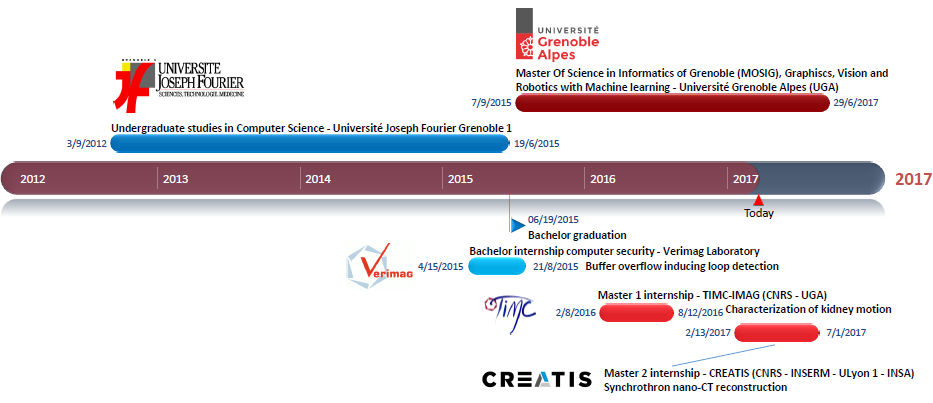
\includegraphics[width=\textwidth]{FriseEtudes.png}

\end{frame}

%------------------------------------------------
%\section{CREATIS M2 project} 
\section{Context of the M2 project}
\begin{frame}
	\frametitle{Context of the M2 project}
	Osteoporosis study:
	
%	\noindent\begin{minipage}{0.3\textwidth}% adapt widths of minipages to your needs

%	\end{minipage}%
%	\hfill%
%	\begin{minipage}{0.7\textwidth}\raggedleft
	\begin{itemize}
		\item Bone disease denoted by a loss of bone mass leading to bone deformation and increase of bone breaking risks.
		\begin{center}
			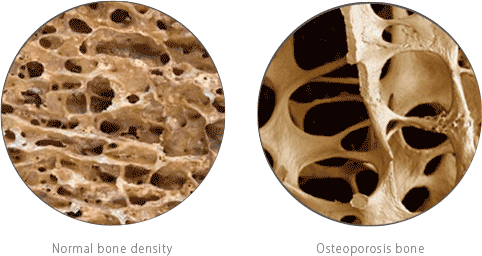
\includegraphics[width=4cm]{bone.png}		
		\end{center}
		\item Interest in 3D nano-scale resolution imaging that is crucial to understand the disease.
		
  		
	\end{itemize}
	
%	\end{minipage}
	\frametitle{Context of the M2 project}
	

\end{frame}

\begin{frame}

\begin{itemize}
		\item Synchrotron nano-CT could be used \textbf{but radiation dose at
this resolution is too high (affects the sample)}\\
  $ \rightarrow $ Need of low-dose methodology (acquisition protocols and algorithms)
  		\item (-) No much work on low-dose synchrotron nano-CT
  		\item \textbf{Objective:} Provide a scalable algorithm for low-dose Synchrothron Nano-CT and validate on bone data.
\end{itemize}

\end{frame}




\section{Previous work}
	
\begin{frame}
\small
	\frametitle{Objective and previous work (1)}
		 Douglas splitting and wavelet shrinkage on Micro-SR-CT imaging\footcite{[2]}. Using 270 of 1800 projections to reconstruction with a resolution of $18 \mu m$. 
		 
	\begin{center}
			
\includegraphics[width=10cm]{2.png}		
		\end{center}
\end{frame}

\begin{frame}
	\frametitle{Objective and previous work (2)}
	Use of ordered subset intensity-based maximizing the a posteriori (OS-iMAP)\footcite{[19]}. From 1500 projections reconstruct using 100 of them with a resolution of $0.5 \mu m$.
		\begin{center}
			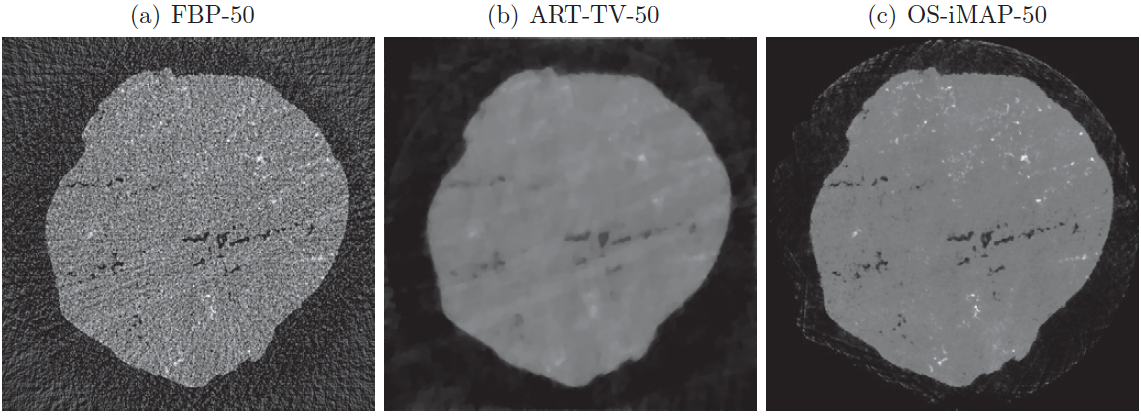
\includegraphics[width=10cm]{19.png}		
		\end{center}
	
\end{frame}

\section{M2 Project plan}

\begin{frame}
	\small
	\frametitle{M2 Project plan}
	Data set:
	\begin{itemize}
		\item Synchrotron nano-CT images of a bone sample of resolution $120 nm$ with 2000 projections ($2048 \times 2000$) 
		\item Multiple reconstruction senarios with different number of projections and noise $\rightarrow$ low-dose simulation
	\end{itemize}
	Method:
	\begin{itemize}
		\item splitting methods (split Bregman, ART + denoising).
		\item investigate regularization functionals (bone detail preservation).
		\item Scalability and eficiency, exploiting ESRF facilities PyHST2\footcite{mirone2014pyhst2}.
	\end{itemize}
	
\end{frame}


\end{document}

\begin{frame}
\small
\frametitle{References}
\bibliographystyle{abbrv}
\bibliography{biblio.bib}
\end{frame}
